\subsection{ Parte estrutural do sistema}

 O material escolhido para a estrutura foi o compensado, as chapas de compensado são materiais versáteis e amplamente utilizados na indústria da construção, marcenaria e artesanato. Elas são fabricadas a partir de finas lâminas de madeira, conhecidas como lâminas de folheado, coladas umas sobre as outras com fibras perpendiculares, conferindo maior estabilidade e resistência mecânica ao produto final, Figura \ref{fig3:image_02}.

\begin{figure}[!h]
	\centering
	\caption{Chapas de compensado.}
	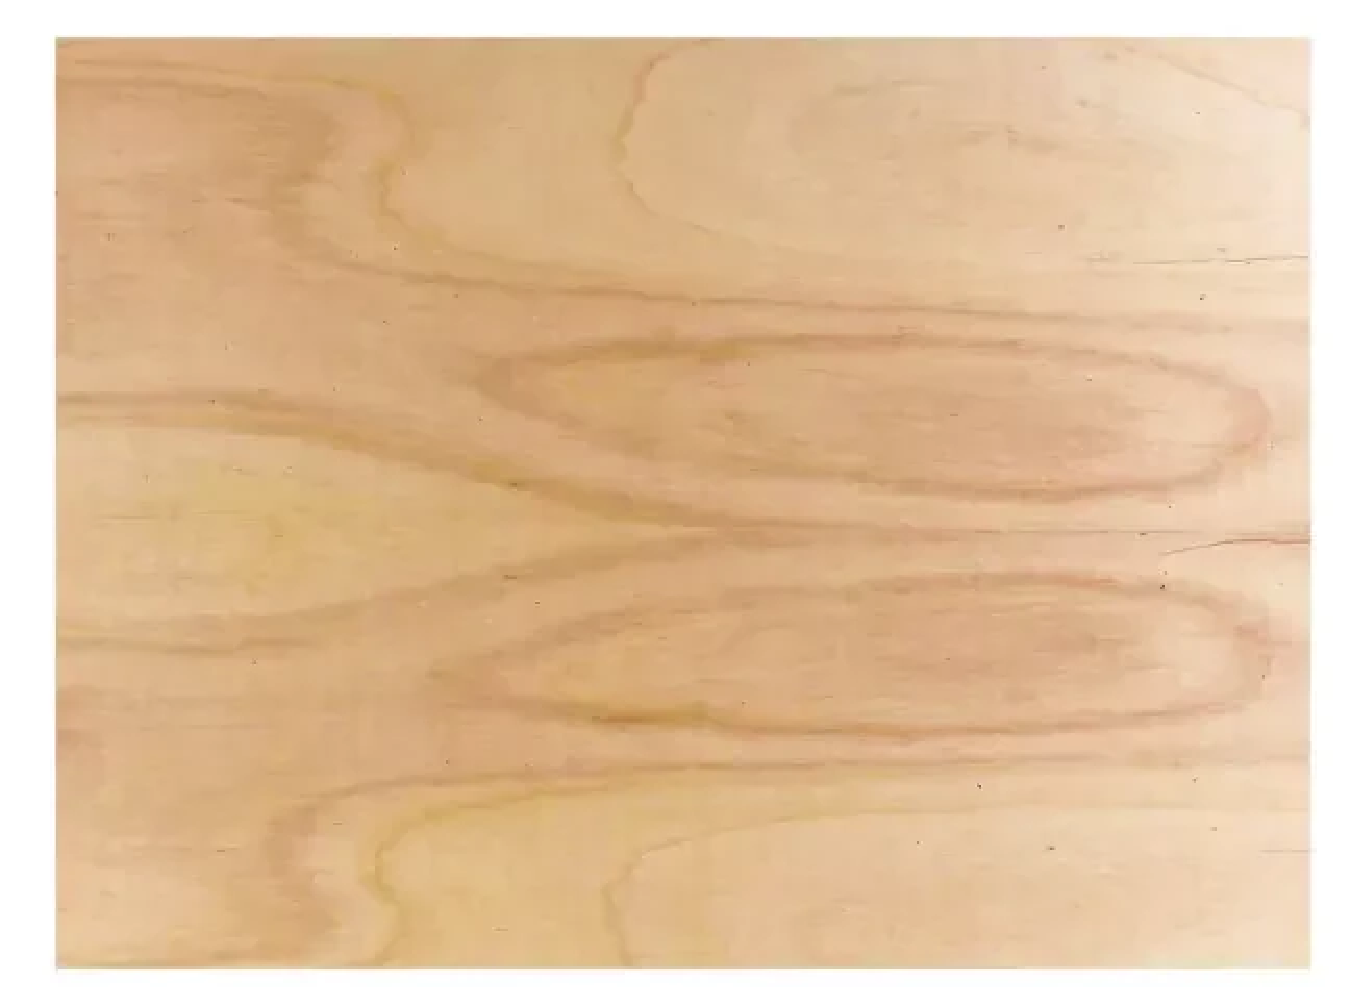
\includegraphics[width=0.6\textwidth]{Capitulos/3_simulacao_e_prototipo/3_figuras/compensado.eps}
	\caption*{Fonte $-$ Autor.}
	\label{fig3:image_02}
\end{figure}



 Já para o braço do Aeropêndulo foi usando Tubo de Fibra de Vidro de Carbono 3x3x2mm, Figura \ref{fig3:image_03}.

\begin{figure}[!h]
	\centering
	\caption{Tubo de Fibra de Vidro de Carbono 3x3x2mm.}
	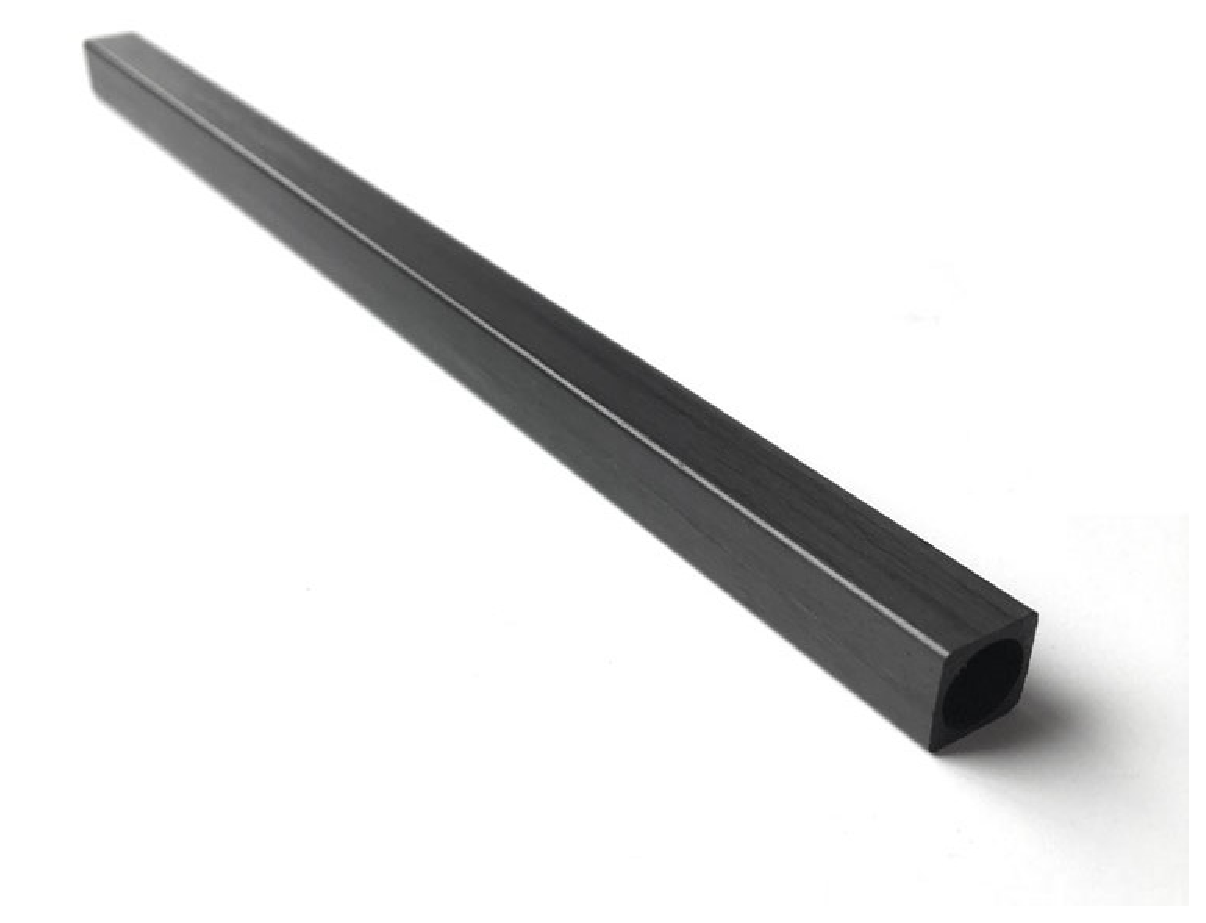
\includegraphics[width=0.5\textwidth]{Capitulos/3_simulacao_e_prototipo/3_figuras/carbono2x2mm.eps}
	\caption*{Fonte $-$ Autor.}
	\label{fig3:image_03}
\end{figure}


\subsection{Parte Elétrica do sistema}

Os componentes eletrônicos usados foram 1 Potenciômetro $50k\Omega$, 1 Placa de desenvolvimento Esp32, 1 Módulo Driver L298n, 
Conjunto suporte motor cw/ccw hélice para drones fpv racing quadcopter e componentes eletrônicos (resistor, capacitor).

\subsubsection{Potenciômetro $50k\Omega$}

O potenciômetro e o \textit{enconder} para se obter o ângulo do braço do Aeropêndulo, isso é possível, pois a medida que o braço se move, a resistência do potenciômetro varia e com ela a tensão nos terminais dele, com isso é possível obter uma relação entre a variação da tensão e o ângulo do braço do Aeropêndulo.

\begin{figure}[!h]
	\centering
	\caption{Potenciômetro $50k\Omega$.}
	\includegraphics[width=0.5\textwidth]{Capitulos/3_simulacao_e_prototipo/3_figuras/pote.eps}
	\caption*{Fonte $-$ Autor.}
	\label{fig3:image_04}
\end{figure}




\subsubsection{Placa de desenvolvimento Esp32}

A placa de desenvolvimento ESP32 é uma poderosa e versátil plataforma que integra o popular microcontrolador ESP32 desenvolvido pela empresa  \textit{Espressif}. Projetada para atender às demandas de projetos de Internet das Coisas (IoT) e aplicações de conectividade sem fio, a ESP32 oferece uma vasta gama de recursos e funcionalidades. Equipada com um processador dual-core de 32 bits, Wi-Fi, Bluetooth, interfaces GPIO, I2C, SPI e UART, bem como suporte para memória externa, essa placa é um verdadeiro trampolim para desenvolvedores que desejam criar soluções conectadas de forma eficiente. Além disso, a ESP32 possui uma comunidade ativa de desenvolvedores, uma ampla documentação e é compatível com várias plataformas e ambientes de desenvolvimento, tornando-a uma escolha de primeira linha para aqueles que desejam embarcar em projetos inovadores e robustos de IoT.

\begin{figure}[!h]
	\centering
	\caption{Placa de desenvolvimento Esp32.}
	\includegraphics[width=0.5\textwidth]{Capitulos/3_simulacao_e_prototipo/3_figuras/f1_esp32.eps}
	\caption*{Fonte $-$ Autor.}
	\label{fig3:image_05}
\end{figure}


\subsubsection{Fonte Chaveada 2A, 5V, 25W}

\begin{figure}[!h]
	\centering
	\caption{Fonte Chaveada 2A, 5V, 25W.}
	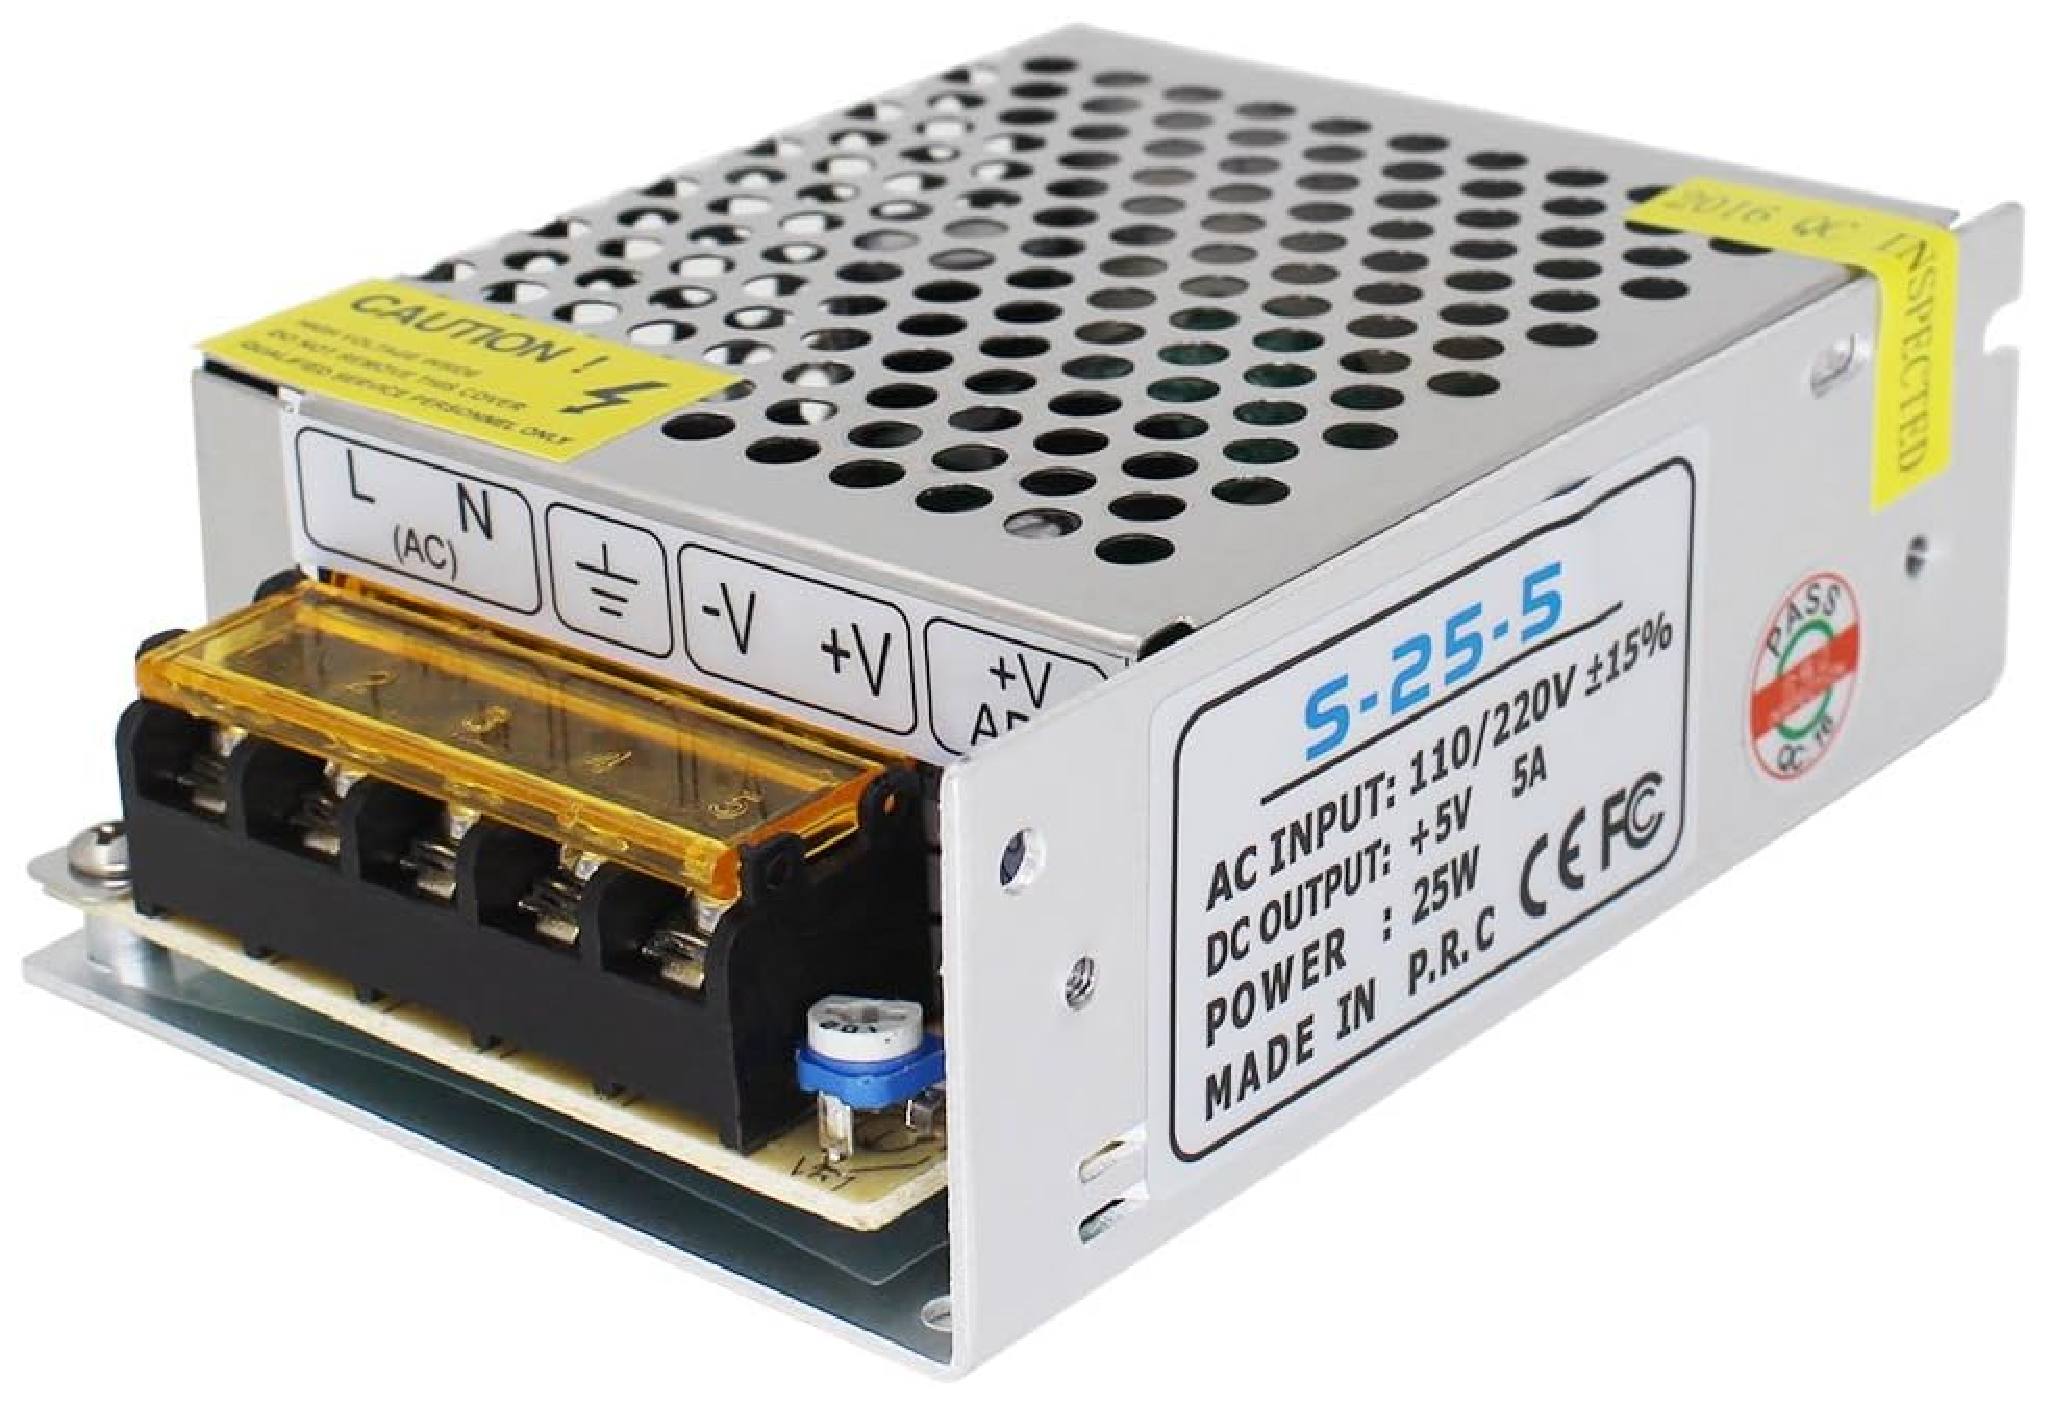
\includegraphics[width=0.5\textwidth]{Capitulos/3_simulacao_e_prototipo/3_figuras/f1_fonte.eps}
	\caption*{Fonte $-$ Autor.}
	\label{fig3:image_06}
\end{figure}

\subsubsection{Módulo Driver L298n}

\begin{figure}[!h]
	\centering
	\caption{Módulo Driver L298n.}
	\includegraphics[width=0.5\textwidth]{Capitulos/3_simulacao_e_prototipo/3_figuras/f4_ponteH.eps}
	\caption*{Fonte $-$ Autor.}
	\label{fig3:image_07}
\end{figure}


\subsubsection{Conjunto suporte motor cw/ccw hélice para drones fpv racing quadcopter}

\begin{figure}[!h]
	\centering
	\caption{Conjunto suporte motor cw/ccw hélice.}
	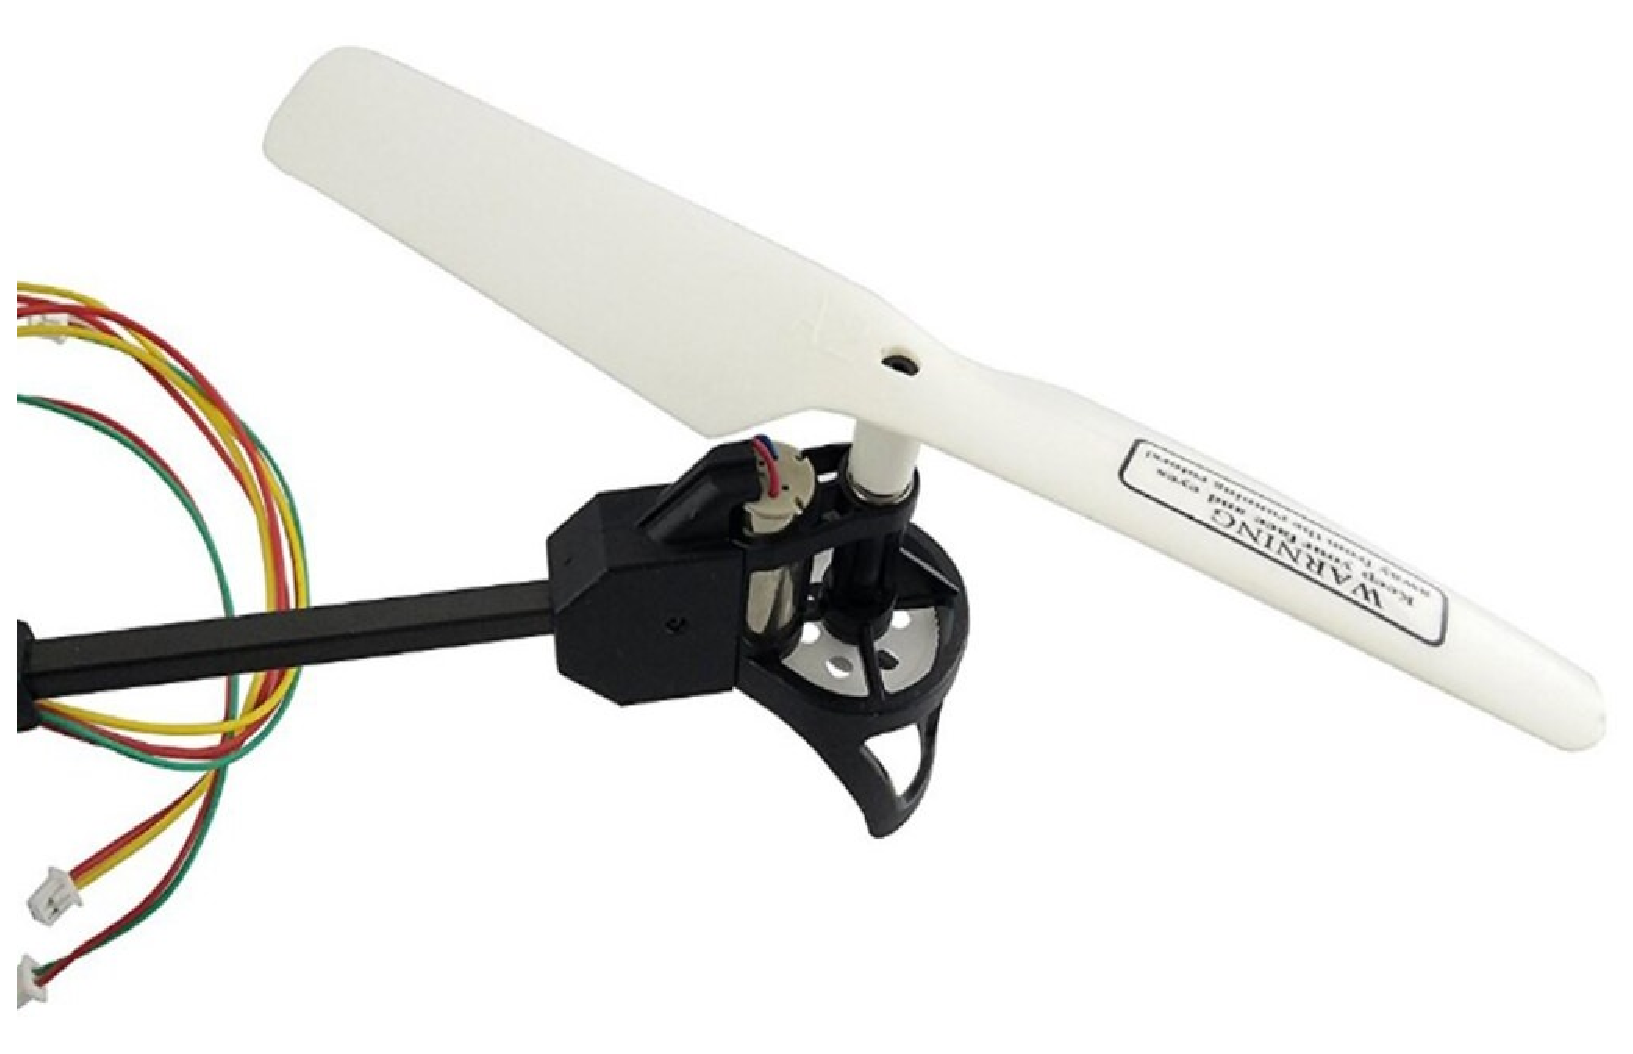
\includegraphics[width=0.6\textwidth]{Capitulos/3_simulacao_e_prototipo/3_figuras/f1_braco_aerop.eps}
	\caption*{Fonte $-$ Autor.}
	\label{fig3:image_08}
\end{figure}

\subsubsection{Componentes eletrônicos (resistor, capacitor)}

\begin{figure}[!h]
	\centering
	\caption{componentes eletrônicos (resistor, capacitor).}
	\includegraphics[width=0.5\textwidth]{Capitulos/3_simulacao_e_prototipo/3_figuras/f1_cap.eps}
	\caption*{Fonte $-$ Autor.}
	\label{fig3:image_09}
\end{figure}



\subsection{Montagem do Protótipo}